%
% The standard LaTeX article class is close to what is needed for an MPhys project report
\documentclass[12pt]{article}

% The following package makes the necessary tweaks to comply with the formatting requirements.
% It also provides a standardised title page, and will warn you if the main text is too long.
\usepackage{mphysproject}
%
%% DO NOT GO CHANGING THE FONT SIZE OR MARGINS! If your main text doesn't fit within 50 pages,
%% you will have to cut stuff out.
%
%% REMEMBER: The target length is around 35 pages
%

% The formatting of the document can be enhanced by loading extra packages.
%
% An essential package is `graphicx', which is loaded by the mphysproject package so you don't
% need to load this yourself. This allows you to include figures using the \includegraphics command.
% To get more information about a package, type texdoc <package> on the Unix command line,
% substituting <package> with the name of the package, e.g., texdoc graphicx
%
% For a wider variety of mathematical environments, symbols and formatting options:
%\usepackage{amsmath,amssymb}
%
% If you want to use colour in the text
%\usepackage{color}
%
% If you want to put figures side by side with separate captions
%\usepackage{subfigure}
%
% If you happen to dislike the standard TeX fonts
%\usepackage{times}
%
% If you include any URLs in your text and/or want to make cross-references clickable, include one of the following
% two lines
\usepackage{hyperref}  % This enables hyperlinks but leaves them in black, which is best for printing
%\usepackage[colorlinks=true]{hyperref} % This colours the hyperlinks, which is better for screen reading
% For Bra-Ket notation.
\usepackage{braket}


\begin{document}

\title{Accelerated Dynamics in HMC Simulations of Lattice Field Theory} % Place your project title in here
\author{Jack Frankland} % Put your name here
\supervisor{Dr Brian Pendleton} % Place your principal supervisor here
\supervisor{Dr Roger Horsley} % If you have additional supervisors, list them with separate \supervisor commands
%\date{1st January 2018} % Today's date will appear on the title page by default, but if you want to tie this to a particular date, you can do so here

% Insert your abstract below
\begin{abstract}
The abstract is a short concise outline of your project area, {\bf of no more than 100 words}. Avoid equations and references in an abstract. 
\end{abstract}

% This command is essential to make the title page appear
\maketitle

% This command introduces the Personal Statement
\personalstatement

\textit{In the Project Report, you must submit a `Personal Statement' describing your project. The Personal Statement is to help the assessors understand what the different parts of the report represent in terms of the work you actually did. Inaccuracy in or lack of a Personal Statement may hinder the assessors and therefore lead to a reduced grade, and should be a maximum of about one page.  A real example follows.}

I spent the first 6 weeks meeting regularly with my supervisor and becoming familiar with the equipment I would be using. I needed to learn about the electronic workings of the experimental system and the programming control I would be administering. I found this initially very time consuming but achieved it by working through the manuals for the pieces of equipment I would be using. I also ran and edited C++ code from an existing package I was given by my supervisor. I was fairly unfamiliar with C++ and so running existing code was a good way for me to begin to understand the language and also the way it could be used to control the equipment.

Outside the lab I began reading articles, LHCb manuals and information from the LHCb website that explained the workings of Multi-Anode Photomultiplier Tubes and how they were being incorporated into the LHCb experiment. As work in the lab was very much about coding and electronics at this stage it was easy to lose sight of the overall goal and so researching such topics kept me focused.

There was a problem with the QDC (charge to digital converter) module I was using, but after switching to the other one I was able to progress. I spent the next 5 weeks administering signals to the QDC module with an external pulse generator. This way I could view the pulse with an oscilloscope and manually set the characteristics I wished to use (width, period etc) before interpreting the resulting data. I edited the C++ code in order to produce text files containing information about each pulse of light, or �event�, being administered. This information was in the form of ADC counts (digital conversions of analogue signals).

During this time, and continuing on through the Christmas break, I continued to research MaPMTs. I conducted a literature review and used this to compile the background knowledge section of my report. The LHCb manuals I was given by supervisor proved to be very informative and provided much of the information for this section. I not only focused on MaPMTs but looked into the Hybrid Photon Detector (HPD) models which are currently used in the LHCb experiment and that the MaPMTs are due to replace.

In Semester 2 I was able to use the MaPMT to obtain data. After initially being introduced to the MaPMT by my supervisor, I spent the first week familiarising myself with how it worked. My supervisor helped me set up an LED pulse which was directed to the photocathode surface of the MaPMT. I spent the next 3 weeks adjusting the equipment to cope with the new pulse source and taking data runs. Much of the code I had worked on in Semester 1 was useful here with constant improvements being made throughout the course of the semester.

I spent the next 2 weeks working learning about the graphical tool ROOT and using it to produce histograms of my results. I was continued working on my report with the Experimental Method section coming to form.

The following 2 weeks were spent altering experimental parameters such as the voltage being administered to the MaPMT and producing further histograms. I spent the remainder of my time analysing my histograms and working on my report.

% If you have anyone that needs to be acknowledged (e.g., anyone who provided assistance with your project work,
% provided data etc) please do so here. Delete this (or comment it out) if you have no-one to acknowledge.
\acknowledgments

\textit{Please acknowledge any assistance that you received during your MPhys project from anyone other than your supervisor. Please also disclose here any work conducted by yourself prior to the MPhys project that is relevant to the project (e.g., summer project work). Speak to your supervisor or the course organiser if you are not sure about what might be relevant to include here.}

This document was originally written by Victoria Martin who ran the MPhys Project course before me. I thank her for all the good advice that is contained within. Any bugs in the \LaTeX\ style file are entirely my own.

% This command inserts a table of contents, and sets things up for the main text of your report.
% The page count starts from here. DO NOT DELETE OR DISABLE THIS COMMAND!
\maintext


\section{Introduction}

This section should present a brief motivation for your project work. The main purpose here is to  set out the scientific question you aim to answer in your project, and the reasons why this is of current scientific interest. Try and think of the bigger picture beyond your project work (and make sure you return to this in the conclusion). If appropriate you can also give a summary of the report and what each section contains.

As a guide, this section should be intelligible to other MPhys students doing projects in different areas.


\section{Background}

\subsection{Quantum Mechanics}

In quantum mechanics we are often interested in calculating the path integral:
\begin{equation}
	\label{eq:PathIntegral}
	\braket{x_b,t_b|x_a,t_a} = \int {\cal D} x\left(t\right) \exp{\left(\frac{i}{\hbar} S_M\left[x\left(t\right)\right]\right)}.
\end{equation}

$\braket{x_b,t_b|x_a,t_a}$ is the transition amplitude for a particle in position eigenstate (in the Heisenberg picture) $\ket{x_a,t_a}$ to move to position eigenstate $\ket{x_b,t_b}$; this gives us the probability amplitude of a particle at $x_a$ at time $t_a$ to move to position $x_b$ at time $t_b$. The term on the right of equation \ref{eq:PathIntegral} is known as the ``Fenyman path integral''. The measure $\int {\cal D} x\left(t\right)$ is an integral over all paths between $x_a$ and $x_b$. $S_M\left[x\left(t\right)\right]$ is the Minkowski action of a particle on the path $x\left(t\right)$ and is defined by:
\begin{equation}
	\label{eq:MinkowskiAction}
	S_M\left[x\left(t\right)\right] = \int_{t_a}^{t_b} dt \left[\frac{1}{2}m\left(\frac{dx}{dt}\right)^2 - V(x)\right],
\end{equation}
where $x\left(t_a\right) = x_a$ and $x\left(t_b\right) = x_b$ are the boundary conditions.

Due to the oscillating integrand in equation \ref{eq:PathIntegral}, it is not clear the integral will converge, and the integral measure needs to be defined before we proceed. In order to do this we follow the steps in \cite{creutz_freedman_1981} to get equation \ref{eq:PathIntegral} into a form we can work with. 

The first step is to discretise time as in figure \ref{fig:TimeLattice}.
\begin{figure}
	\centering
	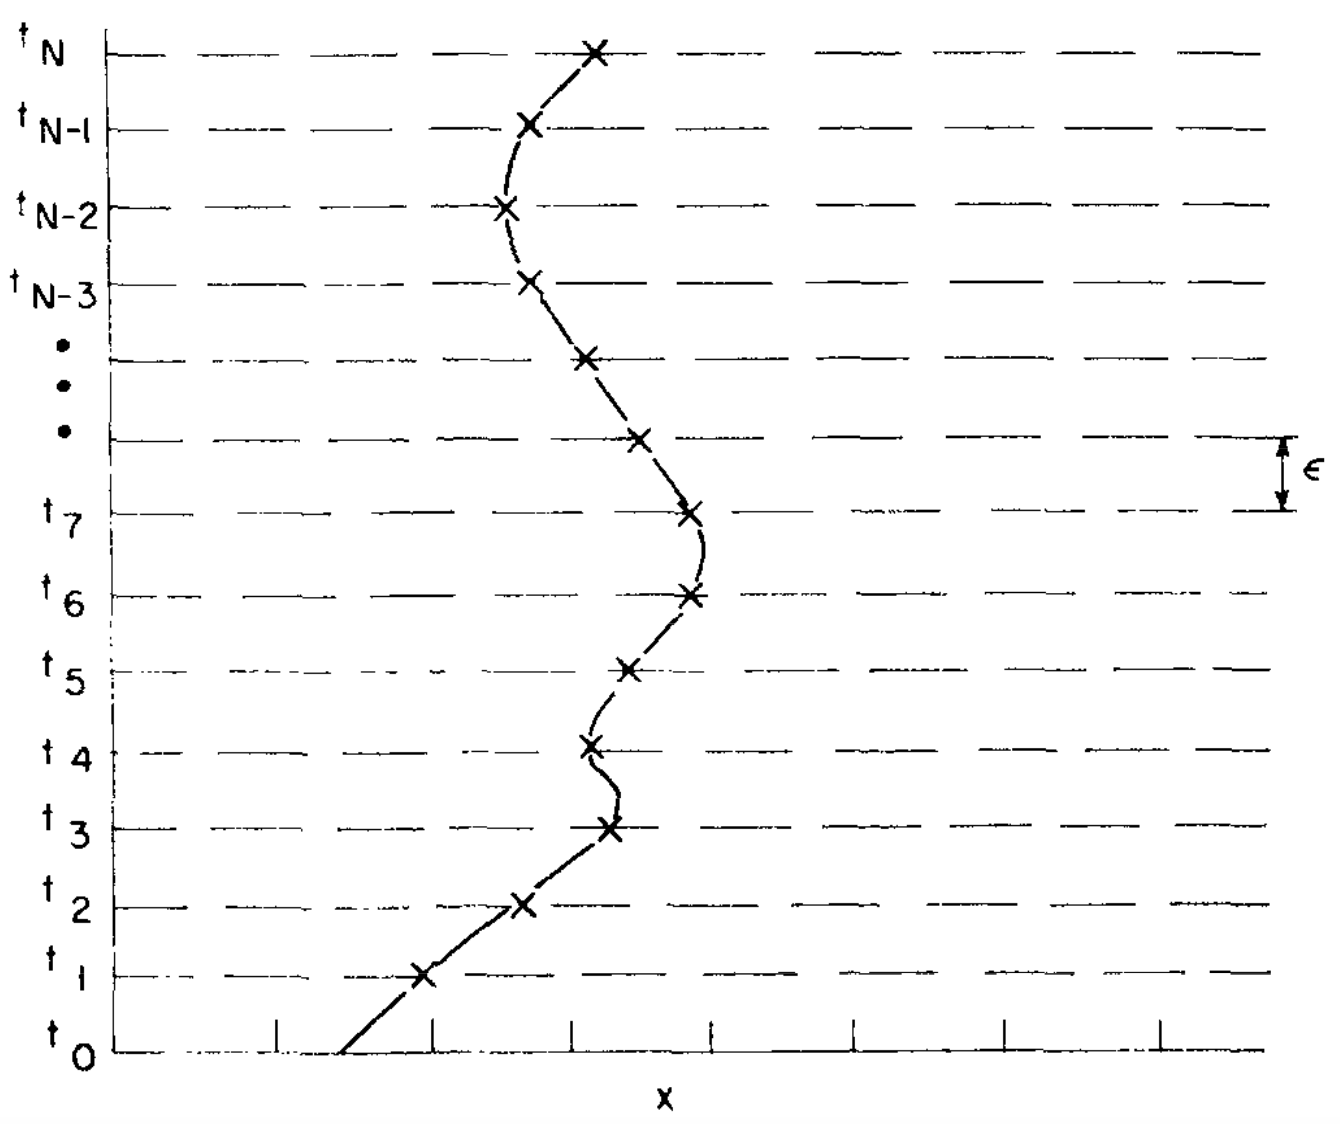
\includegraphics[scale=0.5]{TimeLattice.png}
	\caption{Discretising time into a lattice of spacing $\epsilon$. Diagram taken from \cite{creutz_freedman_1981}}
	\label{fig:TimeLattice}
\end{figure}
Then for each time site on the lattice $t_i$ we have a position $x_i = x\left(t_i\right) \forall i \in \left[0,N\right]$. In our notation for the labelling of the position eigenstates in equation \ref{eq:PathIntegral} we also have $x_b=x_N=x\left(t_N\right)$ and $x_a=x_0=x\left(t_0\right)$ in order to match with figure \ref{fig:TimeLattice}. $ \epsilon $ is the spacing between lattice sites and so $\epsilon = \frac{t_b-t_a}{N} = t_{i+1}-t_i$ and for $k \in \left[0,N\right], t_k = t_a + k \epsilon $. In order to discretise the action in equation \ref{eq:MinkowskiAction} we approximate the derivative by a forward difference and the integral as a Rieman sum, taking the lattice spacing as our small parameter:
\begin{equation}
	\label{eq:DiscreteMinkowskiAction}
	S_{M}\left\{x_i\right\} = \sum_{i=0}^{N-1} \epsilon \left[\frac{1}{2}m\left(\frac{x_{i+1}-x_{i}}{\epsilon}\right)^{2} - V\left(x_i\right)\right].
\end{equation}

Since $\forall i \in \left[1,N-1\right], -\infty < x_i < \infty$ we may define the measure in equation \ref{eq:PathIntegral} as:
\begin{equation}
	\label{eq:IntegralMeasure}
	\int_{x_a}^{x_b} {\cal D} x = \lim_N{\rightarrow \infty} A_{N}\prod_{n=1}^{N-1}\int_{-\infty}^{\infty}dx_n,
\end{equation}
where $A_N = \left(\nu \left(\epsilon\right)\right)^{N}$ and $\nu \left(\epsilon\right)$ is a normalisation factor on each discrete interval. So that for our discrete time lattice, the path integral is given by:
\begin{equation}
	\label{eq:DiscretePathIntegral}
	\braket{x_b,t_b|x_a,t_a} \sim \int^{+\infty}_{-\infty}\prod_{i=1}^{N-1}dx_i \exp{\left(\frac{i}{\hbar}S\left\{x_i\right\}\right)}.
\end{equation}
In the limit that $N\rightarrow \infty$ (or equivelantly $\epsilon \rightarrow 0$) we recover equation \ref{eq:PathIntegral} from equation \ref{eq:DiscretePathIntegral} exactly. 

In order to work with the discrete path integral in equation \ref{eq:DiscretePathIntegral} we have one final step. We make a ``Wick rotation'' into imaginary time; this is done via the substitution:
\begin{equation}
	\label{eq:WickRotation}
	t = i\tau.
\end{equation}
Defining $a=i\epsilon$ we now have a lattice in imaginary time, of lattice spacing $a$, substituting a into equation \ref{eq:DiscreteMinkowskiAction}:
\begin{equation}
	\label{eq:DiscreteEuclideanAction}
	S_M\left\{x_i\right\} = \sum_{i=0}^{N-1} \epsilon \left[\frac{1}{2}m\left(\frac{x_{i+1}-x_{i}}{\epsilon}\right)^2 + V(x_i)\right] = iS_E\left\{x_i\right\}.
\end{equation}
The quantity $S\left\{x_i\right\}$ is the discretized ``Euclidean'' action; it has this name because the effect of the Wick transformation is that it turns the Mikowski metric $\left(ds_{M}\right)$ into the Euclidean metric $\left(ds_{E}\right)$ on the coordinates $\left(x,y,z,\tau\right)$ and visa-versa:
\begin{equation}
	\label{eq:MetricTransform}
	 ds_{M}^{2}= -\left(dt\right)^2 + \left(dx\right)^2 + \left(dy\right)^2 + \left(dz\right)^2 = \left(d\tau\right)^2 + \left(dx\right)^2 + \left(dy\right)^2 + \left(dz\right)^2 = ds_{E}^{2}.
\end{equation}
This is a very useful result since upon substitution into the discrete path integral in equation \ref{eq:DiscretePathIntegral} we find:
\begin{equation}
	\label{eq:DiscreteEuclideanPathIntegral}
	\braket{x_b,t_b|x_a,t_a} \sim \int^{+\infty}_{-\infty}\prod_{i=1}^{N-1}dx_i \exp{\left(\frac{-1}{\hbar}S_{E}\left\{x_i\right\}\right)}.
\end{equation}
This is known as the discrete euclidean path integral and it far better defined since the ``integrand'' is now exponentially suppressed. We are now able to make a connection to statistical mechanics that enables us to compute the values we want in later sections. We have the standard result from statistical physics that for a system with $N-1$ degrees of freedom labelled by $x_i$ for $i \in \left[0,N-1\right]$ then the partition function is given by:
\begin{equation}
	\label{eq:PartitionFunction}
	Z \sim \int


\section{Methods}

A very important part of your report is a readable description, in standard scientific language, of the method by which the work was carried out. There is an art to getting the level of detail right. You should focus on the philosophy of the approach used and those parts of the methods that are specific and/or highly relevant to the work that you actually did, particularly where some new approach was tried. However please note: this section should not be a  blow-by-blow account of what you did throughout the project. It should {\bf not}  contain large detailed sections about things you tried and found to be completely wrong! However, if you find that a technique that was expected to work failed, that is a valid result and should be included. Also, very standard techniques in your research field should not be written out in detail, but should instead be summarised with appropriate references cited when the reader needs more detail. 

In computational projects you should set out the numerical algorithms in a way that would allow a reader to construct their own implementation. A copy of the actual code could be included in the appendices, but if the code is very long this is unlikely to be helpful. Code snippets, on the other hand (e.g., detailing the main update loop of a simulation code), might be instructive. You might also consider archiving your code, for example, using the University's DataShare service. Speak to your supervisor about this.

In theoretical projects, it may not be straightforward to distinguish `methods' from `results' if your method is a calculation. Nevertheless, it would be appropriate to set out the general strategy for performing the calculations (particularly if they are quite involved) before launching into the details. Also, when you get to the end, you will have to explain what your calculations mean.

In general, make sure that the structure you choose is logical and fits your project. Sometimes you you may find that to maintain good structure you may have to present the experiments in a different order from the one in which you carried them out. Some projects naturally divide into multiple separate investigations; for example, an experimental study followed by the development of a theory that is motivated by the experiment. In this case it would be sensible to present the experimental methods and results first; and then a separate set of theoretical methods and results. Discuss the most appropriate report structure with your supervisor.


\section{Results and Discussion}

This section should detail the results obtained in a clear, easy-to-follow manner. It is important to  make clear what are original results and what are repeats of previous experiments or benchmarking. Remember long tables of numbers are just as boring to read as they are to type-in, so use graphs to present your results wherever practicable. Make sure that all tables and figures are actually referred to in the text (see Table~\ref{tab:atable} and Figure~\ref{fig:cmbr} for examples).  Experimental and simulation results should be presented with uncertainties (errors), both statistical and systematic where applicable.

\begin{table}[htb]
\begin{center}
\begin{tabular}{l|l|l}
Particle type & Spin & Multiple occupancy allowed \\\hline\hline
Bosons & Integer & Yes \\
Fermions & Half-integer & No \\\hline
\end{tabular}
\end{center}
\caption{\label{tab:atable} Summary of the key properties of fermions and bosons.}
\end{table}


Be selective in what you include. For example, half a dozen tables that contain wrong data you collected while you forgot to switch on the power supply are not relevant and may mask the correct results. Similarly, you may have made a lot of experimental measurements or generated a lot of simulation data sets that show more or less the same thing. Choose one or two representative examples, and explain in the text the conditions under which similar results were obtained, rather than painstakingly setting out large numbers of figures that add little additional value to the report.

\begin{figure}[htb]     %Insert a figure as soon as possible
\begin{center}
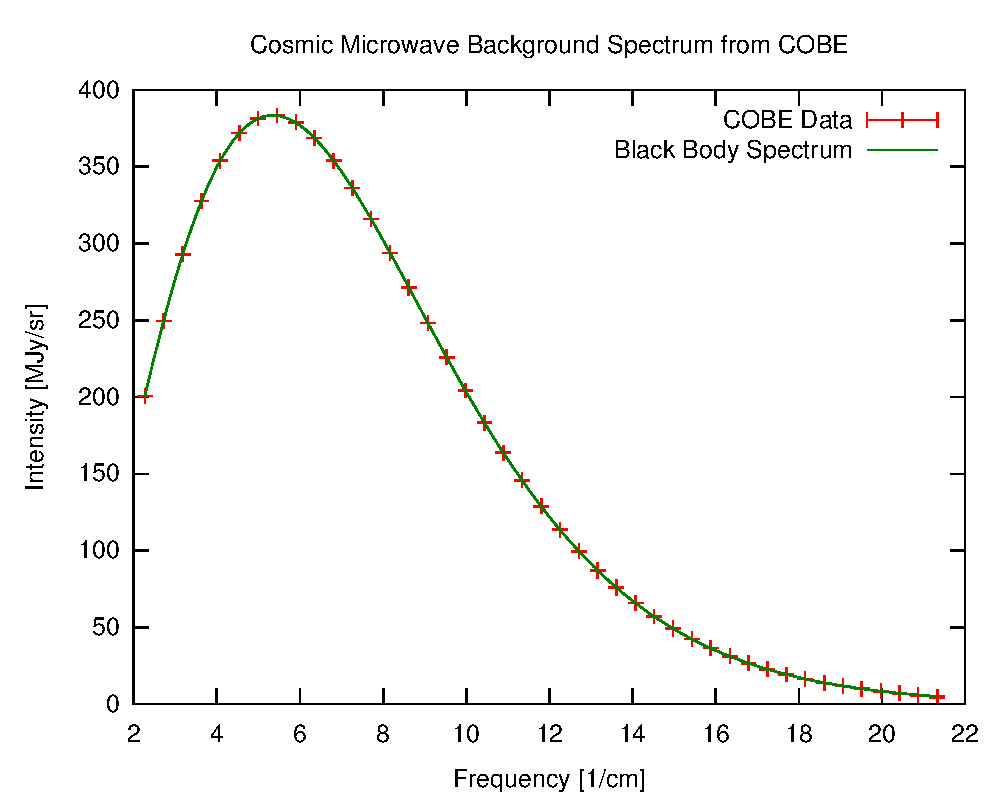
\includegraphics[width=10cm]{Cmbr} % Vary the value in the width=XX setting to resize the figure if need be.
\end{center}
\caption{\label{fig:cmbr} The cosmic microwave background radiation spectrum, a figure that was taken from Wikipedia \cite{wk:cmbr}. The line is the theoretical prediction, and the crosses are observational data (errors are smaller than symbol size). Note the close correspondence between the two. Make sure that all text on the figure is legible at the size the figure is included at. Note in general it is bad practice to have a title on the graph, as here, as the caption is supposed to describe the figure. The caption should also draw the reader's attention to the specific feature(s) of interest (which, here, is the close correspondence between observation and theory). Don't forget to label axes, ideally with words, rather than just symbols.}
\end{figure}

Your report  must contain a discussion of the results. This should include a discussion of the experimental and/or numerical errors, and a comparison with the predictions of the background and theory underlying the techniques used. This section should highlight particular strengths and/or weaknesses of the methods used.


\section{Conclusion}

The first part of a conclusion typically summarises the main results that have been obtained and the conclusions you drew from them. This will probably be a precis of the more detailed discussion in the previous section. This small amount of mild repetition helps to reassure the reader that they agree with you about what the main project findings are.

In the conclusion, you should also place your results into context, for example, by linking back to the original motivating questions posed in the introduction. Furthermore, some discussion of the limitations of the conclusions and suggestions for future work would be appropriate here.

The conclusion section should be 1--2 pages long.


\section{References}

Detail the relevant references which should be cited at the correct place in the text of the report. There are no fixed rules as to how many references are {\it needed}. Generally the longer the project, and the more background reading you had to do, the more references will be required. 

Follow the style of references usually used in your research field.

Generally for a journal article give {\it Author}, {\it Title of article}, {\it Journal Name}, {\it Volume}, {\it Page}, and {\it Year}; for a book give, {\it Author}, {\it Title}, {\it (Editor if there is one)}, {\it Publisher}, and {\it Year}; for a website give the url and the date you accessed the information.

Please note that websites are not always the most appropriate reference, please check if the same information is originally from a journal article or book.

The list of references that appears below is automatically generated using a tool called BibTeX: see Appendix~\ref{sec:bibtex}.

\subsection{Tips on avoiding unwitting plagiarism}

You may well find that published papers, particularly review articles, contain good explanations of the background and methods relevant to your project. Do not be tempted to copy or paraphrase these explanations. They will be picked up by Turnitin, and you may find your work referred for investigation by an Academic Misconduct Officer, which clearly you want to avoid at this stage in your degree.

The golden rule is \emph{always to write in your own words}. My approach is to read through a paper and extract the salient points that are relevant, and then to attempt to write my own account without directly referring to the source (except to check technical points for correctness). If you are following, for example, a derivation or a description of an experimental protocol, you may find it hard to deviate in substance from what has been written elsewhere. In such situations, you should make absolutely clear that you are following this existing presentation, e.g., with phrases like ``We briefly summarise the argument set out in \cite{phd:blythe}, and refer the reader to this work for more details.'' It is also helpful sometimes to note what you have expanded, suppressed or modified, e.g., with phrases like ``An account of this technique is given in \cite{phd:blythe}. That discussion focussed more on the mathematical properties of the probability distribution: here we focus more on how to apply it.'' What this then says to the reader is that we may expect some similarities in the more mathematical parts, but you are adding your own insights by focussing on applications.

Every project is unique, and so the background section should be tailored to your project. You know which topics are important, so you should summarise your own understanding of these, citing references when you are quoting established facts or results, pointers for further reading, or to establish key (often, the earliest) contributions in the field. I have a rule of thumb that when citing a paper as part of a longer discussion about the development of the field, you should write a sentence stating what the authors aimed to achieve in their paper, and a sentence summarising the main result. Sometimes, these can be combined into a single sentence. For example, ``In \cite{phd:blythe}, the reaction dynamics was related to a matrix ordering problem, which was then solved to show that the density decays either exponentially or as a power law depending on the model parameters.''

There are some situations where it is acceptable, and indeed advisable, to include material from other works verbatim. These include:
\begin{itemize}
\item verbal arguments whose precise wording is extremely important. In such cases you should place quotation marks around the source material or,
\begin{quotation}
for longer quotations use a `block-quote' format, as shown here, with the source material cited at the end. \cite{meta}
\end{quotation}
When quoting text, you \emph{must} reproduce exactly what is written. If you need to edit the text, for example, so that it makes grammatical sense in the context of your prose, use [square brackets] to show where words have been added or replaced, and ellipses \ldots to show where words have been deleted.
%
\item technical figures, for example, those showing original data. Redrawing or recreating somebody else's scientific data (e.g., experimental measurements) would be akin to passing it off as your own, so here you should simply include the relevant figure in your own text. Such figures are usually covered by copyright, so technically one is supposed to obtain permission from the publisher when this is down. In any case, you should always included a reference to the source image (e.g., the paper it appears in), e.g., ``taken from \cite{wk:cmbr}'' if included without change or ``adapted from \cite{wk:cmbr}'' if you have made modifications.

For more schematic figures (e.g., a flow chart illustrating a simulation algorithm, or a diagram of an experimental set-up or physical principle) you are usually best off drawing your own, as then labels etc can be tailored to your project (e.g., by using the same terminology). It will be assumed that where figure captions do not cite a source, the figure is entirely your own work.
%
\item structured content, like tables. In some cases, you may find that the material you need to include has been tabulated in an accessible way in another work. Here, the same rules apply as for figures, in that it is acceptable to incorporate this information as long as you include a reference of the form ``taken from \ldots'', ``adapted from \ldots'' in the caption. Again, the absence of a citation sends a message to the reader that you put together all the information that appears in captioned material.
\end{itemize}


% This command tells LaTeX how to format your references in the biblography. The standard plain formatting, with
% references appearing in the order they are cited, is absolutely fine for our needs.
\bibliographystyle{unsrt}

% This command includes the reference list. You will need to compile two or three times (perhaps BiBTeXing after
% the first time) to get the references in synch with the text.
\bibliography{ref,Report}

% This command switches to appendices. The page count ends here.
% NOTE: the material contained in appendices will NOT count towards the assessment of your report.
% Consequently the main text should be self-contained.
\appendix

\subsection*{Explanation of the above note}

The above note will be automatically inserted into your report if you include appendices using the \verb|\appendix| command.

The maximum length of the main text of your report is \textbf{50 pages}, starting from the first word of the introduction and ending with the final reference.  For the avoidance of doubt, the title page, personal statement and table of contents \emph{do not} contribute to the page limit, and nor do any appendices following the main text. These appendices however should not contain any material that is essential to understanding the work that was done in the project, and correspondingly, will not form part of the assessment of the report.

As a rule of thumb, it is legitimate to use an appendix when there is additional information that would be of benefit to a student following on from your project. Under certain circumstances the following might be appropriate:
\begin{itemize}
\item Intermediate steps of routine algebra that could not be reproduced by a competent Honours-level student without any specific hints as to the path to follow.
\item Fragments of computer code where the implementation details are of importance.
\item Diagrams of experimental apparatus built, or detailed specification of the instruments used.
\item Specialist data tables used to analyse results.
\item Photographic plates.
\end{itemize}

\section{\LaTeX\ hints and tips}

If you have not used \LaTeX\ before, you may find its philosophy confusing to begin with. Basically, you describe to \LaTeX\ the content you want to appear in your report, and it then goes and works out how to typeset it. This means, for example, that \LaTeX\ will automatically number sections, position figures, maintain cross-references and so on for you. Be prepared for a lot of work if you want to deviate from the layout it produces. In most cases, the choices it makes are good ones.

There are a number of good \LaTeX\ tutorials on the web, a good place to start is to Google `latex tutorial'. There are a few common pitfalls that I mention here for reference:
\begin{itemize}
\item In \LaTeX\ you need to explicitly type open and close quotes as distinct characters. An open quote (`) is typed using the \verb|`| character, and a close quote (') is typed with the \verb|'| character. If you need double quotes, you need to double up these characters: \verb|``like this''| gives you ``like this''.
\item You can label most numbered object, for example, sections, subsections, tables, figures, items in a numbered list, equations, etc, using \verb|\label{|\textit{key}\verb|}|, putting a useful shorthand name where it says \textit{key}. When you want to refer to the numbered object, use \verb|\ref{|\textit{key}\verb|}|. You may need to recompile a couple of times to get the labels and keys in synch. The benefit comes when you move things around, split sections into subsections, or join sections together. After a couple of recompiles, your crossreferencing has sorted itself out.
\item \LaTeX\ automatically places extra space after full stops. This gives a more pleasing appearance to paragraphs of text. However, a full stop does not always indicate the end of a sentence, e.g.~following the abbreviation `e.g.'. The simplest way to get a normal-sized space is to use a \verb|~| character. This also prevents a line-break at this position. Many people put such a non-breaking space when citing figures and tables: see Fig.~\ref{fig:cmbr}, which is typed as \verb|Fig.~\ref{fig:cmbr}|. Even if you write out Figure in full, this will stop the figure number appearing at the start of a line, which looks odd to some people.
\item Use the \texttt{graphicx} package (included automatically if you use the \texttt{mphysproject} style sheet) to include graphics using the \verb|\includegraphics| command. There is an example in the source of this document for you to see how it works.
\end{itemize}

\LaTeX\ really comes into its own when it comes to including equations in your report. The rest of these tips concern equations.
\begin{itemize}
\item There are two (main) ways to include equations. The first is to include them inline. For example, Newton's second law can be written as $F = ma$, which is typeset as \verb|$F = ma$|. A single dollar sign opens and closes an inline equation. The second type of equation is a displayed equation. For example, the partition function of the quantum mechanical harmonic oscillator is
\begin{equation}
Z(1) = \frac{{\rm e}^{-\frac{\hbar\omega}{2kT}}}{1 - {\rm e}^{-\frac{\hbar\omega}{kT}}} \;.
\end{equation}
In the source document, this equation is written as
\begin{verbatim}
\begin{equation}
Z(1) = \frac{
  {\rm e}^{-\frac{\hbar\omega}{2kT}}}
}{
  1 - {\rm e}^{-\frac{\hbar\omega}{kT}}}
} \;.
\end{equation}
\end{verbatim}
\item There are many mathematical symbols you can include: tables of these symbols can be found by doing a Google search on `latex math symbols'. Sometimes you need to include additional packages (like \texttt{amsmath} or \texttt{amssymb}) to use more exotic symbols.
\item If you have brackets around sums, integrals, fractions or other large objects, use \verb|\left| and \verb|\right| so that they are automatically made large enough to enclose their contents. Compare for example
\begin{equation}
\left( \sum_{k=0}^{\infty} z^k \right) \;,
\end{equation}
typeset as \verb|\left( \sum_{k=0}^{\infty} z^k \right)|, as opposed to
\begin{equation}
( \sum_{k=0}^{\infty} z^k ) \;,
\end{equation}
which does not use \verb|\left| or \verb|\right|.
\item The mysterious error `You cannot use \verb|\eqno| in math mode' means that you have forgotten a \verb|\right| that is needed to match a \verb|\left|.
\item Always use the \verb|\begin{equation}| \ldots \verb|\end{equation}| environment for displayed equations, rather than one of the other options available to you. This makes sure that an equation number appears. Even though you may not refer to a particular equation, someone else might want to!
\item Equations should be punctuated as normal text. So if a displayed equation ends a sentence, place a full stop at the end of it. It helps to insert a little bit of spacing, using \verb|\;| before this punctuation.
\item It is tempting in the source to insert blank lines before and after equations for readability. Do not do this, as this starts a new paragraph (inserting extra space) each time. Only put a blank line if the paragraph has genuinely ended.
\item Some people insist that exponential ${\rm e}$ and total derivatives ${\rm d}$ should be set in roman font using \verb|{\rm e}| and \verb|{\rm d}| whilst others find this overly fussy.
\item However, everyone agrees that you should set things like $\sin x$ and $\cos x$ using \verb|\sin x| and \verb|\cos x| and not as \verb|sin x| and \verb|cos x|, as the latter come out as $sin x$ and $cos x$: that is, these read as the variable $s$ times $i$ times $n$ times $x$ and as $c$ times $o$ times $s$ times $x$, and not what you actually want.
\item Finally, one for statistical physicists. The ensemble average of a quantity, $E$, say, is written as \verb|\langle E \rangle|, which gives you $\langle E \rangle$ (and not \verb|<E>| which gives you the much more ugly $<E>$). You might prefer to use overbars which avoids this problem. Ask your supervisor about any typesetting conventions that are peculiar to your field. 
\end{itemize}

\section{\LaTeX\ vs pdf\LaTeX}

Traditional \LaTeX\ generates what is known as a \texttt{.dvi} file, which is somewhat peculiar to the \TeX\ ecosystem. In particular, if you use \LaTeX\ you need your figures to be in PostScript format, and after compiling your document you will need to convert it to PDF.

Most people these days instead use pdf\LaTeX\ which uses PDF as its file format all the way through. You can include figures in PDF, JPEG and PNG format directly into pdf\LaTeX\ documents using the \verb|\includegraphics| command. If you have figures in other formats, the \texttt{convert} utility on Linux machines will be able to convert to PDF, e.g., using \texttt{convert myfigure.xpm myfigure.pdf}.

\section{BibTeX}
\label{sec:bibtex}

It is most convenient to use \texttt{bibtex} to compile your bibliography. First you need to create a \texttt{.bib} file. For example, you may call it \texttt{ref.bib}.

Then you can put all your references into the file with entries such as
\begin{verbatim}
@Book{ob:bornwolf,
     author = "Born, M and Wolf, E",
     title  = "Principles of Optics",
     publisher = "Cambridge University Press",
     year = 1999,
     edition = {7th},
}

@Article{jr:ashkin,
Author = {A. Ashkin and J.M. Dziedzic and J.E. Bjorkholm and S. Chu},
Title = "Observation of a single beam gradient force optical tap for 
dielectric particles",
Journal = "Optics Letters",
Volume = 11,
Pages = "288-290",
Year = 1986}

@INPROCEEDINGS{seger,
 author = {J. Seger and H.J. Brockman},
 title = {What is bet-hedging?},
 editors={P.H. Harvey and L. Partridge},
 booktitle = {Oxford Surveys in Evolutionary Biology},
 year={1987},
 page={18},
 publisher={Oxford University Press},
 place={Oxford}}
\end{verbatim}
for a book, an article in a journal or an article in a proceedings volume respectively.

Inside your latex file you should include 
\begin{verbatim}
\bibliographystyle{unsrt}                      
\end{verbatim}
and
\begin{verbatim}
\bibliography{ref}
\end{verbatim}
The first command determines the reference style, here plain and unsorted. With this referencing style a numerical referencing system (which is the most common in physics literature) is used and the numbering of references will be the order in which they appear in the document. The second command just inputs your .bib file. Note that only the references cited in the text will appear in the bibliography so you can have spare references in your \texttt{.bib} file.

You use the name you have given to an entry (e.g.~for the book example above the name is \verb|ob:bornwolf|) to cite the relevant article by using the cite command in your latex file e.g.~\verb|\cite{ob:bornwolf}|.

The process by which \LaTeX\ builds the reference list is a bit complicated. If you have not compiled a document before, or have made changes to which references are cited since you last compiled, you will need to execute the following (assuming you are using pdf\LaTeX):
\begin{verbatim}
  pdflatex ProjectReport
  bibtex ProjectReport
  pdflatex ProjectReport
  pdflatex ProjectReport
\end{verbatim} 
This first time you run \texttt{pdflatex}, it works out all the references you have cited (along with other items you have labelled for crossreferencing, and what should go in the table of contents) and puts all this information into a file called \texttt{ProjectReport.aux}. The bibliography itself needs to be constructed using this information from the \textit{ref.bib} file, which you do by running \texttt{bibtex}. (The bibliography itself lands in a file called \texttt{ProjectReport.bbl}). When you next run \texttt{pdflatex} command, the bibliography is appended to your document---but until this happens \LaTeX\ doesn't know which number each reference should have. This information will by now be in the \texttt{ProjectReport.aux} file, so when you next run \texttt{pdflatex} the correct numbers will be inserted. If you are really unlucky, the formatting of the document will have caused some changes to the document that will necessitate another run of \texttt{pdflatex}. Pay attention to the messages that appear when you compile, and make sure that the message `There were undefined references' does not appear (you might need to scroll up a bit to check for this).

If you don't change any references, then it will generally be sufficient to run \texttt{pdflatex} once to compile the document.  Before submission, I would run the entirety of the sequence above to avoid any last-minute cross-referencing errors, with one more run of \texttt{pdflatex} for luck.


\end{document}